\newpage

\lhead{\leftmark}
\chapter{Planning and Architecture}

\cfoot{\thepage}

\parindent=0.5in
\onehalfspacing
\section{Introduction}
The success of any project depends on the quality of its initiation. This chapter is dedicated to the analysis and specification of requirements for our project. We will begin by identifying the stakeholders, then discuss the functional and non-functional requirements of the project, introduce use case diagrams, present the product backlog, and conclude with the solution architecture and our working environment.

\section{Stakeholder Identification}
A stakeholder represents an external entity that interacts with the system, such as a human operator or another system. They can consult or modify the system state, which in response to a stakeholder's action, provides a service corresponding to their need. Based on this definition, our application has 4 main stakeholders:\vspace{0.5cm} \newline

- Administrator: \newline He can manage all system functionalities including user management, site configuration, equipment management, and system administration tasks.
\vspace{0.5cm} \newline

- Network Engineer:\newline He can manage sites, equipment, and interventions while having access to technical documentation and system configuration.\vspace{0.5cm} \newline

- Field Technician:\newline He can view assigned interventions, update intervention status, and access site information needed for field operations.
\vspace{0.5cm} \newline

- Manager:\newline He can view reports, monitor system performance, and access management dashboards without modification rights.\newline

\section{Requirements Specification}
After presenting the stakeholders, our next step consists of describing the different functional and non-functional requirements that our application must fulfill.

\subsection{Functional Requirements}
In this section we present the different functional requirements of our application.\vspace{0.5cm} \newline

- Authentication and Authorization :\newline
Allow users to authenticate to access the application.
Manage different authorization levels to access application functionalities.
\vspace{0.5cm} \newline

- Site Management : \newline
Allow users to manage mobile network sites including 2G, 3G, 4G, and 5G installations.
Enable site creation, modification, and status monitoring.
\vspace{0.5cm} \newline

- Equipment Management : \newline
Display existing equipment at selected sites.
Calculate and display total available resources.
Track equipment installation dates and maintenance schedules.
\vspace{0.5cm} \newline

- Intervention Management : \newline
Display scheduled interventions and maintenance activities.
Allow intervention assignment to field technicians.
Track intervention progress and completion status.
\vspace{0.5cm} \newline

- Alert System : \newline
Generate and manage real-time alerts for network issues.
Classify alerts by severity level.
Enable alert acknowledgment and resolution tracking.
\vspace{0.5cm} \newline

- Reporting and Analytics : \newline
Generate reports on site performance and maintenance activities.
Calculate performance indicators and maintenance costs.
Provide data export capabilities.

\subsection{Non-Functional Requirements}
In this section we present the different non-functional requirements of our application.\vspace{0.5cm} \newline

- Interface Ergonomics :\newline The application must be simple, clear, easy to handle and understand, and well organized from a graphical point of view.
\vspace{0.5cm} \newline

- Efficiency and Reliability :\newline The application must satisfy the user and guarantee processing speed.
\vspace{0.5cm} \newline

- Robustness :\newline The program must be able to support loads, store data and ensure good error handling.
\vspace{0.5cm} \newline

- Maintainability :\newline The application is designed, developed and organized in a way that can be easily maintained and improved in the future.
\vspace{0.5cm} \newline

- Security :\newline The application is secured via an authorization process so that data is only accessible to authenticated and authorized users.\newline

\section{Product Backlog}\\
\begin{longtable}{|c|p{4cm}|p{7cm}|c|}
\caption{Product Backlog} \\ \hline
\textbf{ID} & \textbf{Functionality} & \textbf{User Story} & \textbf{Priority} \\ \hline
1 & Authentication & As an admin, engineer, technician, and manager, I can authenticate & High \\ \hline
2 & Manage Sites & As an admin and engineer, I can add, delete, modify and select sites.\vspace{0.25cm} \newline As technician and manager, I can select sites & High \\ \hline
3 & Manage Equipment & As an admin and engineer, I can add, delete, modify and select equipment.\vspace{0.25cm} \newline As technician and manager, I can select equipment & High \\ \hline
4 & Manage Interventions & As an admin and engineer, I can create, modify and assign interventions.\vspace{0.25cm} \newline As technician, I can update intervention status & High \\ \hline
5 & Manage Equipment Types & As an admin, I can view, add, modify and delete equipment type specifications.\vspace{0.25cm} \newline As engineer, technician and manager, I can view equipment type specifications & High \\ \hline
6 & Manage Site Performance & As an admin, I can view, add, modify and delete site performance metrics.\vspace{0.25cm} \newline As engineer, technician and manager, I can view site performance metrics & High \\ \hline
7 & Manage Alerts & As an admin and engineer, I can view, add, modify and delete network alerts.\vspace{0.25cm} \newline As technician and manager, I can view and acknowledge alerts & High \\ \hline
8 & Manage Network Coverage & As an admin and engineer, I can view, add, modify and delete network coverage data.\vspace{0.25cm}  \newline As technician and manager, I can view network coverage data & High \\ \hline
9 & Manage Maintenance Costs & As an admin, I can view, add, modify and delete maintenance cost data.\vspace{0.25cm}  \newline As engineer, technician and manager, I can view maintenance costs & Medium \\ \hline
10 & Manage Service Prices & As an admin, I can view, add, modify and delete service pricing information.\vspace{0.25cm} \newline As engineer, technician and manager, I can view service prices. & Medium \\ \hline
11 & Manage Breakdown Reports & As an admin and engineer, I can view, add, modify and delete breakdown reports.\vspace{0.25cm}  \newline As technician, I can create and update breakdown reports. As manager, I can view breakdown reports. & Medium \\ \hline
12 & Manage Site Monitoring & As an admin and engineer, I can view, add, modify and delete site monitoring configurations.\vspace{0.25cm} \newline  As technician and manager, I can view site monitoring data. & Medium \\ \hline
13 & Manage User Profiles & As an admin, I can view, add, modify and delete user profiles and roles.\vspace{0.25cm} \newline As engineer, technician and manager, I can view and update my own profile. & Low \\ \hline
14 & Manage Performance Reports & As an admin and manager, I can view, add, modify and delete performance reports.\vspace{0.25cm} \newline  As engineer and technician, I can view performance reports. & Low \\ \hline
15 & Generate Analytics & As an admin and manager, I can generate comprehensive analytics and dashboards.\vspace{0.25cm} \newline As engineer and technician, I can view analytics dashboards. & Low \\ \hline
\end{longtable} \newline

\section{Sprint Planning}\vspace{1cm}
For the proper execution of the project, the work will be divided into a certain number of sprints. These sprints are defined using the product backlog, taking into account the priority of the different modules. Given that our project includes business understanding and conceptual design tasks, the first sprint will focus on foundational elements, and the subsequent sprints are presented in the figures below. At the end of each sprint, we will have a release that will be reviewed to plan changes and developments to be carried out in the next sprint.\newline
\begin{figure}[hbt! ]
    \centering
    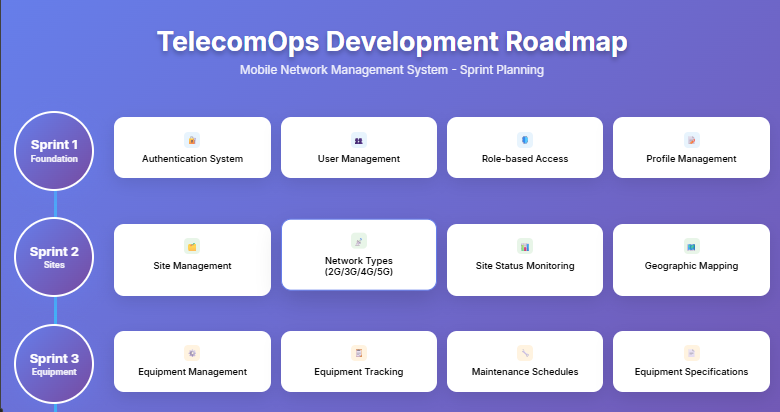
\includegraphics[width=1\linewidth]{img/chap_02/sprints_1_2_3.png}
    \caption{Sprint 1, 2 and 3}
    \label{fig:sprints_123}
\end{figure}
\begin{figure}[hbt!]
    \centering
    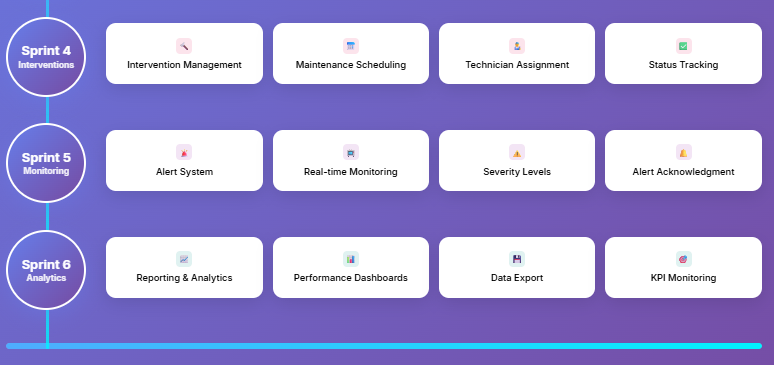
\includegraphics[width=1\linewidth]{img/chap_02/sprints_4_5_6.png}
    \caption{Sprint 4, 5 and 6}
    \label{fig:sprints_456}
\end{figure}\newpage

\section{Global Use Case Diagram}
In this section, we present the global use case diagram of our application.
\begin{figure}[hbt!]
    \centering
    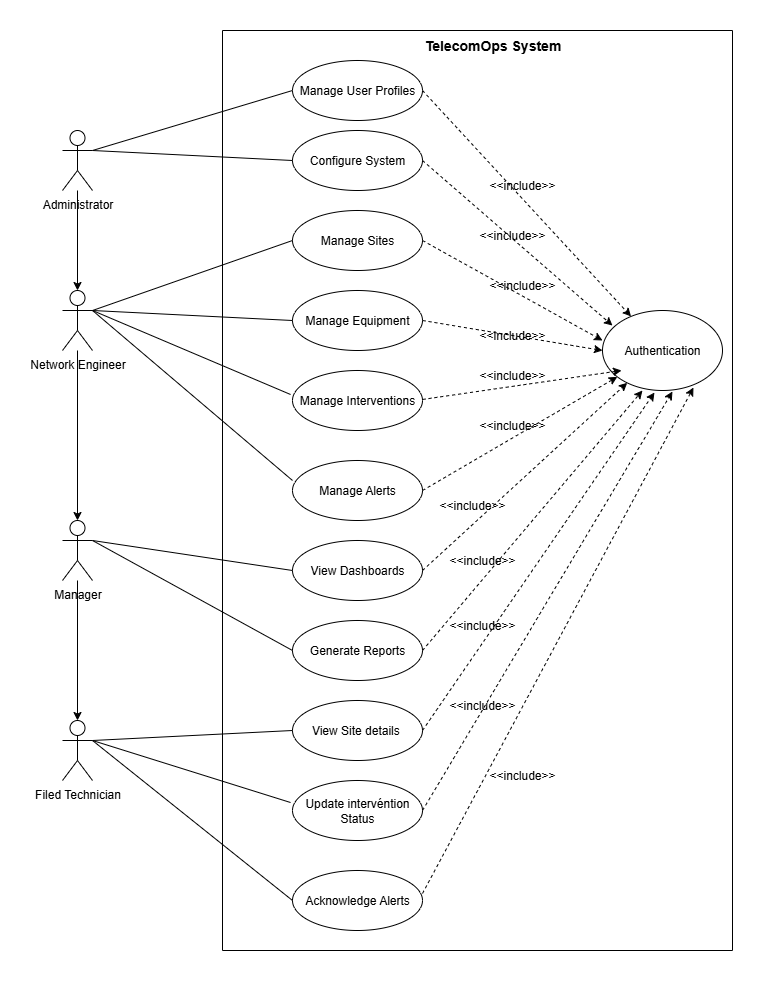
\includegraphics[width=0.95\linewidth]{img/chap_02/TelecomOps_UseCase_Diagram.png}
    \caption{Global Use Case Diagram}
    \label{fig:use_case_global}
\end{figure}\vspace{1cm}

\section{System Architecture}
In this section, we describe the complete system architecture of the TelecomOps application, including the monolithic architecture pattern, technological stack, and deployment strategy.

\subsection{Monolithic Architecture Overview}
The TelecomOps system follows a monolithic architecture pattern where all application components are tightly integrated and deployed as a single unit. This approach provides simplicity in development, deployment, and maintenance while leveraging the full-stack capabilities of Next.js for telecommunications site management.

\begin{figure}[hbt!]
    \centering
    \includegraphics[width=0.9\linewidth]{img/chap_02/monolithic_architecture.png}
    \caption{Monolithic Architecture Components}
    \label{fig:monolithic_architecture}
\end{figure}

\subsection{Architecture Description}
The TelecomOps monolithic architecture integrates all layers within a single Next.js application, providing a unified development and deployment experience for telecommunications operations. All components are packaged and deployed as one unit, simplifying the overall system management.

\subsubsection{Architecture Layers}

\textbf{User Interface Layer:}
The presentation layer built with React components handles all user interactions for site management, equipment tracking, alert monitoring, and intervention scheduling. This layer provides responsive interfaces for our four user roles: administrators, network engineers, field technicians, and managers.

\textbf{Business Logic Layer:}
The business layer contains API routes and server-side functions that implement telecom-specific rules such as site status processing, equipment lifecycle management, alert severity calculations, and maintenance scheduling algorithms. All business logic resides within the same Next.js application context.

\textbf{Data Access Layer:}
The data layer uses Supabase client to interact with the PostgreSQL database. It handles all CRUD operations for sites, equipment, interventions, alerts, breakdowns, and user profiles with Row Level Security policies ensuring proper access control.

\begin{figure}[hbt!]
    \centering
    \includegraphics[width=0.9\linewidth]{img/chap_02/TELECOMOPS_SYSTEM_ARCHITECTURE.png}
    \caption{TelecomOps Monolithic System Architecture}
    \label{fig:system_architecture}
\end{figure}

\subsubsection{Key Architectural Benefits}

The monolithic architecture provides several advantages for the TelecomOps system:

\begin{itemize}
\item \textbf{Development Simplicity:} Single codebase reduces complexity and accelerates feature development for telecom operations.
\item \textbf{Deployment Efficiency:} One build and deployment process simplifies CI/CD pipeline and reduces operational overhead.
\item \textbf{Performance Optimization:} No network latency between layers ensures fast response times for field technicians.
\item \textbf{Data Consistency:} ACID transactions across all features maintain site and equipment data integrity.
\item \textbf{Cost Effectiveness:} Lower infrastructure and operational costs benefit telecommunications operators.
\end{itemize}

\subsection{Technology Stack}
The application utilizes a unified technology stack within the monolithic architecture context:

\begin{itemize}
\item \textbf{Full-Stack Framework:} Next.js 14 with TypeScript
\item \textbf{UI Framework:} React 18 with Tailwind CSS and Shadcn/ui
\item \textbf{Backend Services:} Supabase (Authentication, Database, Real-time)
\item \textbf{Database:} PostgreSQL with Row Level Security
\item \textbf{Deployment:} Vercel Platform with Global CDN
\end{itemize}

\subsection{Database Architecture}
The database schema is designed to efficiently manage telecommunications site data within the monolithic context. All six tables (sites, equipment, interventions, alerts, breakdowns, profiles) are accessed through the same application instance.

\begin{figure}[hbt!]
    \centering
    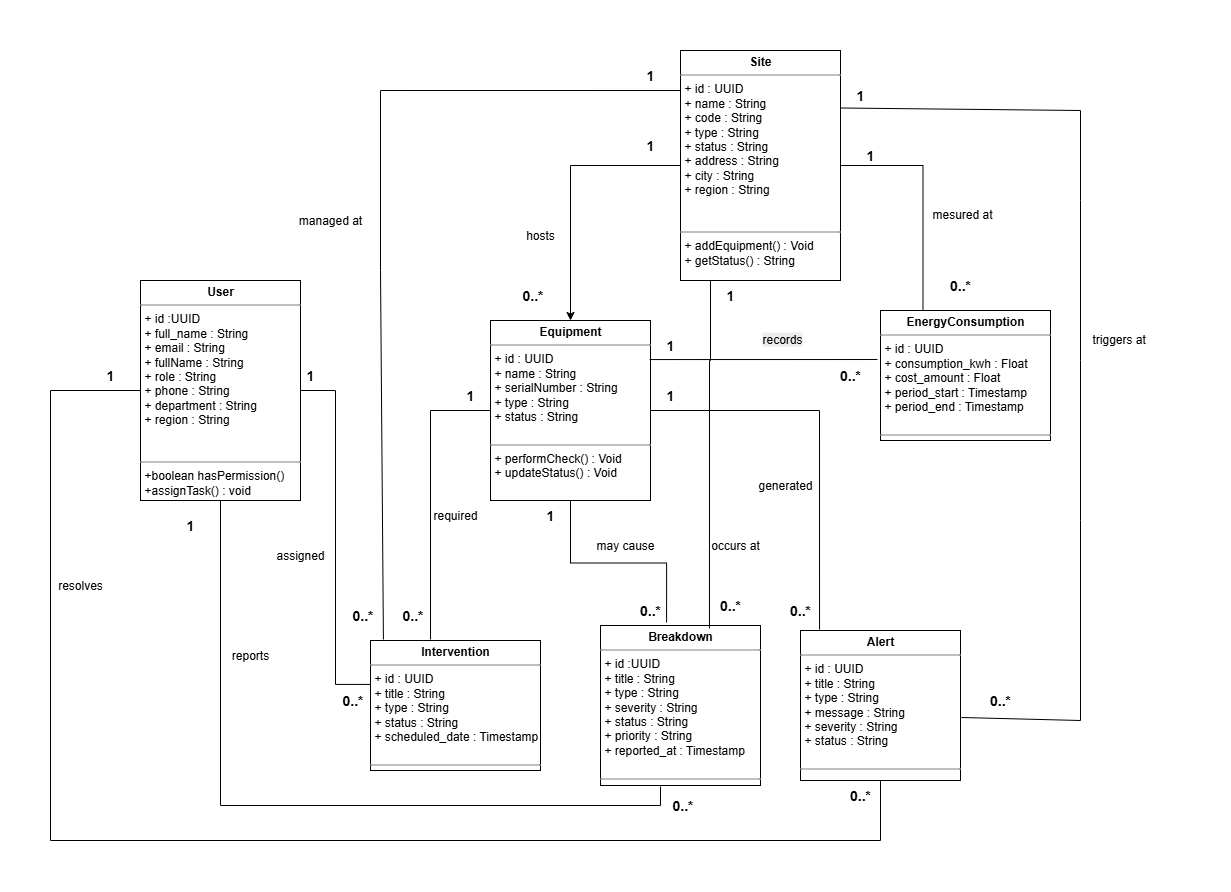
\includegraphics[width=0.85\linewidth]{img/chap_02/database_er_diagram.png}
    \caption{Entity Relationship Diagram}
    \label{fig:database_er_diagram}
\end{figure}

\subsection{Data Flow Architecture}
In the monolithic architecture, data flows seamlessly between layers within the same application context, reducing latency and complexity. All layer interactions occur through direct method calls rather than network requests.

\begin{figure}[hbt!]
    \centering
    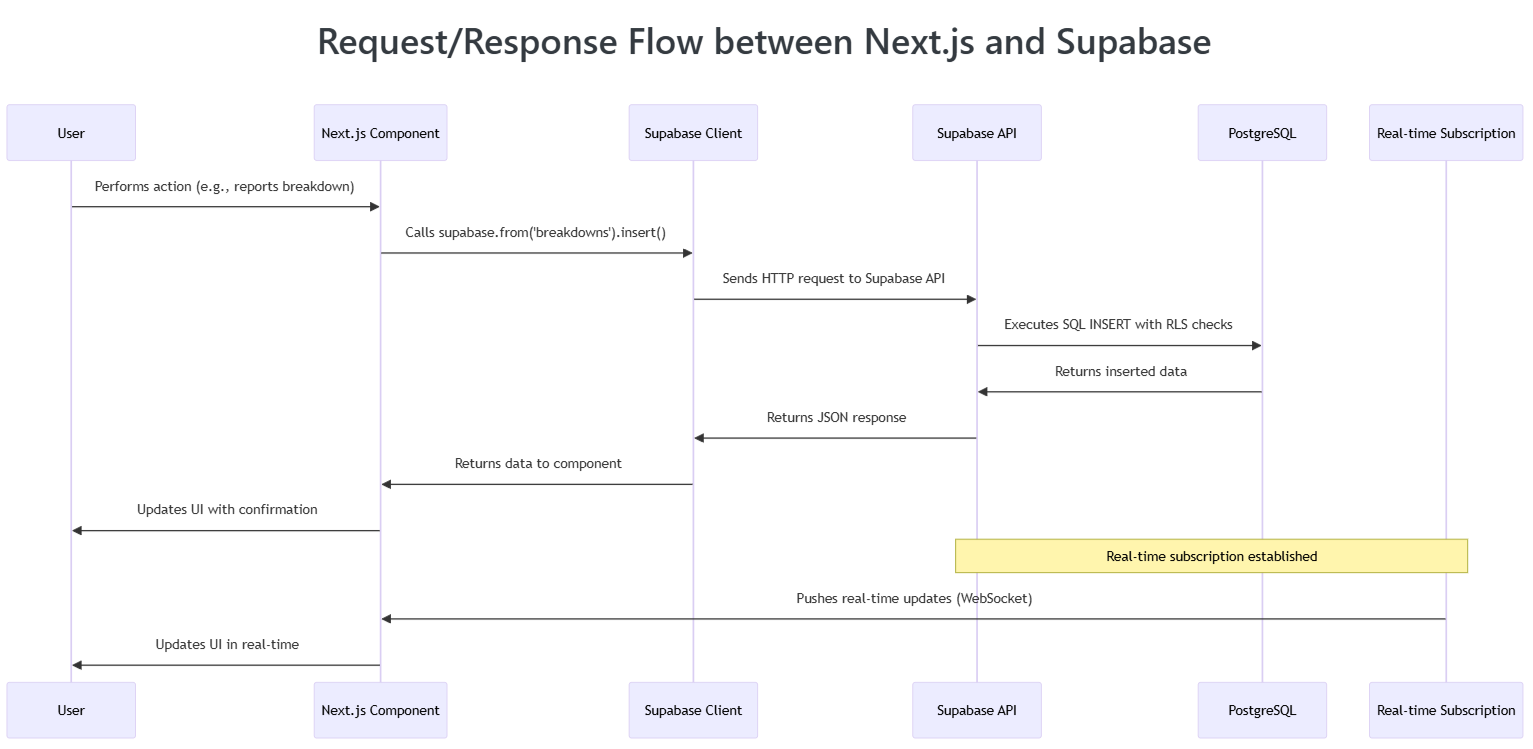
\includegraphics[width=0.9\linewidth]{img/chap_02/data_flow_architecture.png}
    \caption{Monolithic Data Flow}
    \label{fig:data_flow_architecture}
\end{figure}

\subsection{Security Architecture}
Security in the monolithic architecture follows a unified approach with consistent enforcement across all layers. Authentication, authorization, and data security are handled within the same application context.

\begin{figure}[hbt!]
    \centering
    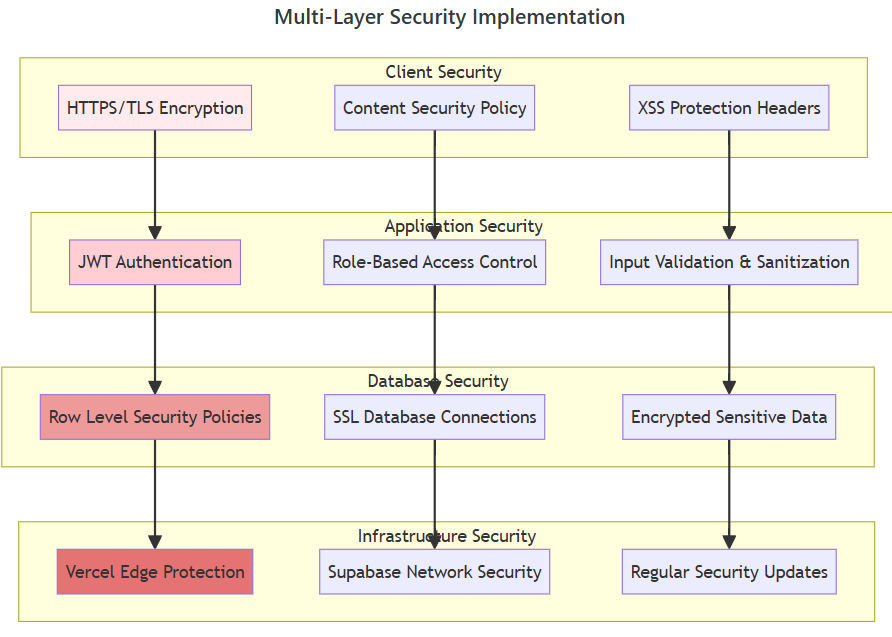
\includegraphics[width=0.9\linewidth]{img/chap_02/security_architecture.png}
    \caption{Monolithic Security Architecture}
    \label{fig:security_architecture}
\end{figure}

\subsection{Deployment Architecture}
The monolithic application deploys as a single unit to Vercel, providing simplified deployment, monitoring, and scaling for telecommunications operations.

\begin{figure}[hbt!]
    \centering
    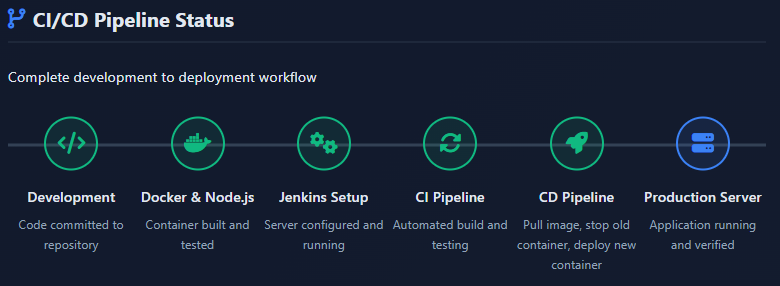
\includegraphics[width=0.85\linewidth]{img/chap_02/deployment_architecture.png}
    \caption{Single Unit Deployment Architecture}
    \label{fig:deployment_architecture}
\end{figure}

\subsection{Why Monolithic Architecture for TelecomOps}
The monolithic architecture is the optimal choice for TelecomOps due to several factors:

\begin{itemize}
\item \textbf{Project Scope:} The well-defined scope of telecom site management fits perfectly within a monolithic structure.
\item \textbf{Team Size:} A small development team can efficiently manage a single codebase.
\item \textbf{Performance Requirements:} Direct method calls provide the fast response times needed by field technicians.
\item \textbf{Data Consistency:} ACID transactions ensure reliable site and equipment data integrity.
\item \textbf{Operational Simplicity:} Telecommunications IT teams prefer simple, maintainable solutions.
\item \textbf{Cost Constraints:} Lower infrastructure costs align with telecom operator budgets.
\end{itemize}

\subsection{Architecture Benefits Summary}
The monolithic architecture provides comprehensive benefits for telecommunications operations:

\begin{itemize}
\item \textbf{Rapid Development:} Faster delivery of site management features
\item \textbf{Simplified Maintenance:} Single application to monitor and update
\item \textbf{Optimal Performance:} No inter-service latency for critical operations
\item \textbf{Clear Architecture:} Easy to understand and extend for new requirements
\item \textbf{Business Alignment:} Matches telecom operational needs perfectly
\end{itemize}

\section{Application Security}
Security is an essential aspect in any web application, especially when it comes to protecting sensitive data and ensuring that only authorized people can access resources. In this project, we have adopted a modern approach to manage user authentication and authorization by integrating Supabase, an open-source Backend-as-a-Service platform.

\subsection{Definition of Supabase}
Supabase is an open-source Backend-as-a-Service platform that provides database, authentication, real-time subscriptions, and API services. It allows centralized management of user identities and access for modern applications.

\subsection{Supabase Security Features}
Supabase ensures unified identity and access management, based on several key features that structure its operation:
\vspace{0.5cm} 
\newline

- User and Role Management: 
\vspace{0.2cm}
\newline
Users are created and managed through Supabase's authentication system and each user can be assigned to one or more roles. Roles determine user permissions in the application based on their job function (Administrator, Network Engineer, Field Technician, Manager).
\vspace{0.5cm}
\newline

- Authentication Process:
\vspace{0.2cm}
\newline
When the user attempts to log in, they interact directly with Supabase's secure authentication service.
After successful login verification, Supabase generates an access token (JWT) containing user information (name, email, role, permissions) and returns it to the application.
\vspace{0.5cm} 
\newline

- Authorization Control: 
\vspace{0.2cm}
\newline
The system verifies the access token received in each request to ensure that the user has the necessary permissions to access the requested resource or perform the requested action.
\newline

\subsection{Interaction with Application Components}
In a modern architecture, interaction between different systems relies on efficient authentication and authorization management. Here is a detailed overview of the flow and integrations necessary to ensure this communication.
\vspace{0.5cm} 
\newline

- Frontend Application : 
\vspace{0.2cm}
\newline
The frontend, developed with Next.js and TypeScript, uses Supabase's JavaScript client library to manage user authentication. When a user attempts to access the TelecomOps application, Supabase checks if they are already logged in. If not, the user is redirected to the secure login interface to enter their credentials. Once authenticated, Supabase returns an access token that the frontend stores securely. This token is then included in requests sent to API endpoints, enabling access to secured telecom operations. This flow ensures centralized authentication and secure communication between different parts of the application.
\vspace{0.5cm} 
\newline

- Backend API System : 
\vspace{0.2cm}
\newline
The backend, built with Next.js API routes, is configured to validate access tokens generated by Supabase using secure server-side libraries. Each request sent to API endpoints must include a valid token in the HTTP header in the form Authorization: Bearer <token>. When receiving a request, the backend decodes this token to verify the user's identity and role-based permissions. Access to different API endpoints (sites management, equipment tracking, interventions, alerts) is then controlled using middleware and Row Level Security policies, ensuring precise authorization control for telecom operations.
\vspace{0.5cm} 
\newline

- Database Security (PostgreSQL) :
\vspace{0.2cm}
\newline
Business data, such as site information, equipment details, maintenance interventions, and network alerts, are stored in a PostgreSQL database managed by Supabase. Supabase ensures security through Row Level Security (RLS) policies that guarantee only authorized requests reach the database based on user roles and permissions. Once these requests are validated, they are processed normally on the PostgreSQL database with additional security layers protecting sensitive telecom infrastructure data.

\subsection{Global Security Flow}
The global security flow described below illustrates the different stages of secure interaction between systems:
\newline
1. The user attempts to access the TelecomOps application via the web interface.\newline 
2. Supabase authenticates the user credentials and generates a secure access token. \newline
3. The frontend sends requests to API endpoints with the access token included. \newline
4. The backend verifies the token with Supabase and authorizes or denies the request based on user roles and permissions. \newline
5. If authorized, the backend executes the telecom operation on PostgreSQL and returns the secure response to the frontend. \newline

\begin{figure}[H]
    \centering
    \includegraphics[width=1\linewidth]{img/architecture/supabase_security_flow.png}
    \caption{Global Security Flow of TelecomOps Authentication}
    \label{fig:security_flow}
\end{figure}

\subsection{Security Benefits}
The Supabase security implementation provides several advantages for the TelecomOps system:
\vspace{0.5cm} 
\newline

- Centralized Security Management: 
\vspace{0.2cm}
\newline
All authentication and authorization logic is handled by Supabase, reducing security complexity and potential vulnerabilities.
\vspace{0.5cm}
\newline

- Role-Based Access Control:
\vspace{0.2cm}
\newline
Different user types (Administrator, Network Engineer, Field Technician, Manager) have appropriate access levels to telecom operations and sensitive network data.
\vspace{0.5cm} 
\newline

- Data Protection: 
\vspace{0.2cm}
\newline
Row Level Security policies ensure that users can only access telecom site data and equipment information relevant to their role and assigned responsibilities.
\vspace{0.5cm} 
\newline

- Secure Communication: 
\vspace{0.2cm}
\newline
All data transmission between components uses encrypted HTTPS connections with JWT token validation for additional security layers.